% IIT Roorkee presentation theme for beamer class used in Latex
%
% Manisha Verma, Department of Mathematics, <mani7dma@iitr.ac.in>
% Sudip Roy, Department of Computer Science and Engineering, <sudiproy.fcs@iitr.ac.in>, <http://faculty.iitr.ac.in/~sudiproy.fcs/>
% Balasubramanian Raman, Department of Computer Science and Engineering, <balarfma@iitr.ac.in>, <https://sites.google.com/site/balaiitr/>
%
% Date: July 23, 2015
% Version 1.0: First public version.
%
% Project slides: Pricing the Hidden Cost of One More Car on Los Angeles Freeways.
% Figures are in figures/ (generated by the project code in github.com/ipsanmoljj/urban_eco).

\documentclass[compress]{beamer}

\usetheme{IITR} % To use the theme of IITR for beamer class in Latex

\usepackage{textpos}
\usepackage[utf8]{inputenc}
\usepackage[T1]{fontenc}
\usepackage{helvet}
\usepackage{amsfonts}
\usepackage{amsmath}
\usepackage{amssymb}
\usepackage{tikz, graphicx}
\usepackage{booktabs}
\usepackage{array}
\newcolumntype{L}[1]{>{\raggedright\arraybackslash}p{#1}}
\usetikzlibrary{arrows.meta, positioning, shapes.geometric}
\setbeamertemplate{navigation symbols}{}
\setbeamertemplate{headline}{}
\setbeamercovered{transparent}
\usebackgroundtemplate{\includegraphics [width=\paperwidth,height=\paperheight]{slide_bg.png}}
\usepackage{url}
\graphicspath{{figures/}}

\definecolor{IITRBlue}{RGB}{26,33,141}
\definecolor{Amber}{RGB}{184,106,0}
\definecolor{Road}{RGB}{60,60,60}
\newcommand{\hl}[1]{{\color{IITRBlue}\textbf{#1}}}

%%%%%%%%%%%%% Title Slide %%%%%%%%%%%%%%%%%
\title{Pricing the Hidden Cost of One More Car}
\subtitle{Congestion tolls on Los Angeles freeways: does the curve shift by hour?}
\author{Ritu Raj \and Rupsa Seth \and Kanwar Anmol Singh}
\date{{\scriptsize\today} \vspace{3em}}
\institute{Urban Economics Course Project\\
Data and code: \url{https://github.com/ipsanmoljj/urban_eco}}
%%%%%%%%%%%%%%%%%%%%%%%%%%%%%%%%%%%%%%%%%%%
\begin{document}
%%%%%%%%%%%%% Title Slide %%%%%%%%%%%%%%%%%
{\usebackgroundtemplate{\includegraphics[width=\paperwidth,height=\paperheight]{titleslide_bg.png}}
\begin{frame}[plain,t]%{INDIAN INSTITUTE OF TECHNOLOGY ROORKEE}
\titlepage
\begin{textblock*}{200mm}(.94\textwidth,-8.75cm)
\includegraphics[height=.98cm]{logo_white.png}
\end{textblock*}
\end{frame}
}
%%%%%%%%%%%%%%%%%%%%%%%%%%%%%%%%%%%%%%%%%%%

%%%%%%%%%%%%% TOC Slide %%%%%%%%%%%%%%%%%
\begin{frame}[t]{Table of Contents}
\tableofcontents
\end{frame}
%%%%%%%%%%%%%%%%%%%%%%%%%%%%%%%%%%%%%%%%%%%

%==========================================================
\section{Introduction}
%==========================================================
\begin{frame}[t]{The problem: one more car}
\begin{itemize}
\item When a driver joins a busy freeway, they slow down \hl{everyone behind them} a little.
\item They feel only their own delay, not the delay they impose on others: the \hl{congestion externality}.
\item Result: busy roads are \hl{overused}, especially at rush hour.
\item Textbook fix (Pigou): charge each driver a toll equal to the \hl{marginal external cost} (MEC), the delay cost one extra car imposes on all other drivers.
\end{itemize}
\vspace{0.5em}
\begin{block}{Two things we need to know to set the toll}
\begin{enumerate}
\item How much does one extra car actually slow traffic? (causal, not correlation)
\item Should the toll change by the hour, and \emph{why}?
\end{enumerate}
\end{block}
\end{frame}

\begin{frame}[t]{Research question}
\begin{block}{Question}
Is rush hour expensive because \hl{more cars} use the same road, or because the \hl{road itself behaves differently} at rush hour?
\end{block}
\vspace{0.3em}
\begin{columns}[T]
\begin{column}{0.48\textwidth}
\begin{block}{(a) Same curve}
Peak hours just sit further along \emph{one} speed--density curve.\\[0.3em]
$\Rightarrow$ price by how crowded the road is \emph{right now}.
\end{block}
\end{column}
\begin{column}{0.48\textwidth}
\begin{block}{(b) Shifting curve}
The curve itself moves with the clock (driver mix, ramp metering, incidents).\\[0.3em]
$\Rightarrow$ hour-of-day tolls justified on their own.
\end{block}
\end{column}
\end{columns}
\vspace{0.5em}
\small Setting: Caltrans District 7 (Los Angeles and Ventura counties), January--September 2026.
\end{frame}

%==========================================================
\section{Literature}
%==========================================================
\subsection{Findings, methods and empirics}
\begin{frame}[t]{Parry (2009): the theory}
\begin{columns}[T]
\begin{column}{0.5\textwidth}
\small
\begin{itemize}
\item \hl{Optimal toll = MEC}:\\ $\text{MEC} = \text{VOT}\cdot V \cdot \frac{\partial T}{\partial V}$
\item Evaluate it at the \hl{post-toll} traffic level: tolls push drivers off, so the toll is \emph{below} MEC at today's traffic.
\item Needs a \hl{demand response}, unobservable before tolling $\Rightarrow$ report a range.
\item A toll that \hl{varies with congestion} beats a flat charge.
\end{itemize}
\end{column}
\begin{column}{0.48\textwidth}
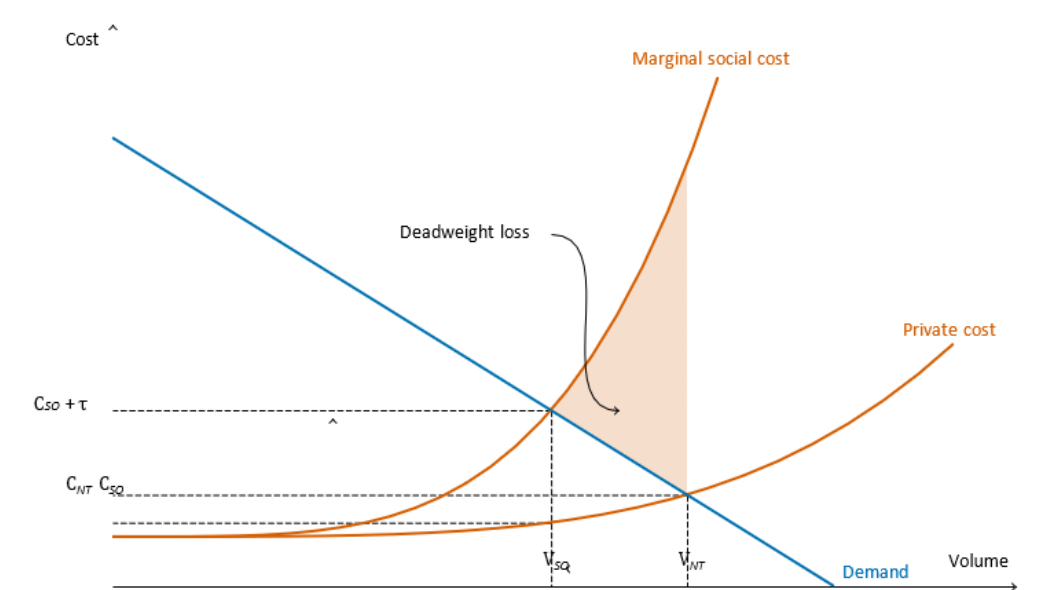
\includegraphics[width=\textwidth]{lit_bento_fig1_standard_model.png}\\
\tiny The standard model: drivers see only the private cost; the toll $\tau$ closes the gap to the marginal social cost and removes the deadweight loss. Source: Bento et al. (2023), Fig.~1.
\end{column}
\end{columns}
\vspace{0.4em}
\begin{block}{What we take}
\small The MEC framework, post-toll evaluation, and the flat vs time-varying comparison.
\end{block}
\end{frame}

\begin{frame}[t]{Bento et al. (2023): method}
\small
\begin{columns}[T]
\begin{column}{0.46\textwidth}
\textbf{Data:} PeMS hourly data, 1,318 mainline stations, Los Angeles (D7), 2017; CHP incidents; Google Maps routes for a 1\% sample of LODES commutes.\\[0.5em]
\textbf{Method}
\begin{itemize}
\item Instrument: a crash on an \hl{alternative route} pushes drivers onto the studied road
\item Speed flat below a \hl{kink}, chosen by AIC: 21 cars/mile/lane
\item 2SLS above and below the kink; station, hour, day, month FE
\end{itemize}
\end{column}
\begin{column}{0.52\textwidth}
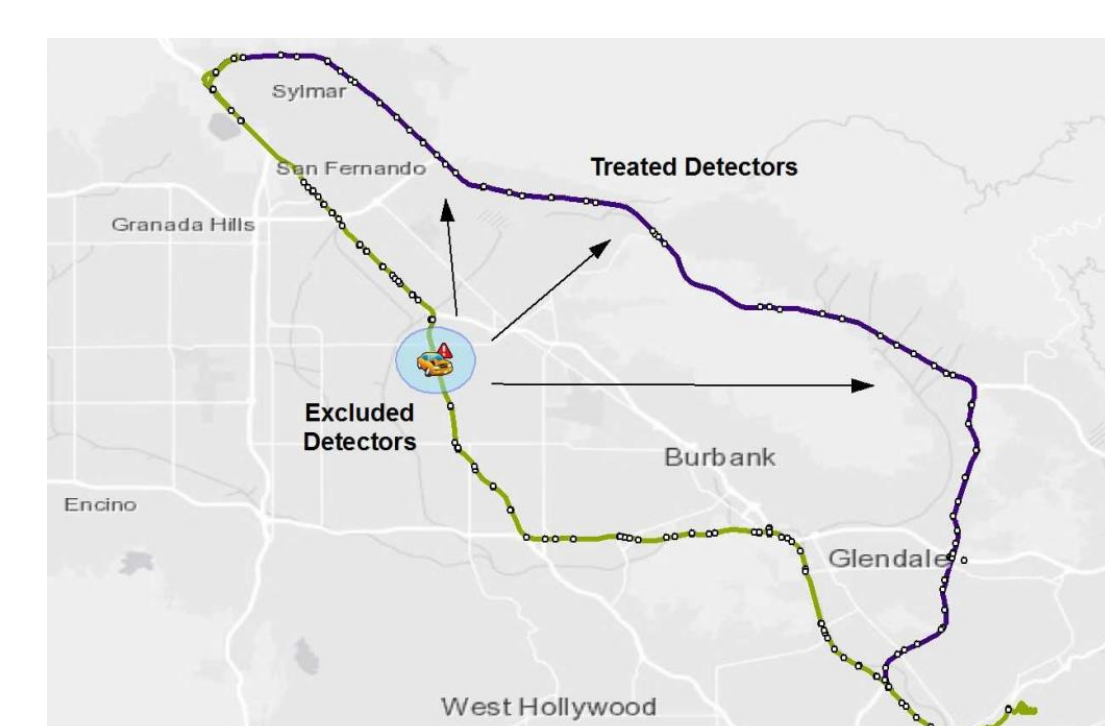
\includegraphics[width=\textwidth]{lit_bento_fig8_instrument.png}\\
\tiny A crash on the green route: detectors on the blue alternative become ``treated''; detectors on the crash's own link are excluded. Source: Bento et al. (2023), Fig.~8.
\end{column}
\end{columns}
\end{frame}

\begin{frame}[t]{Bento et al. (2023): findings}
\small
\begin{columns}[T]
\begin{column}{0.56\textwidth}
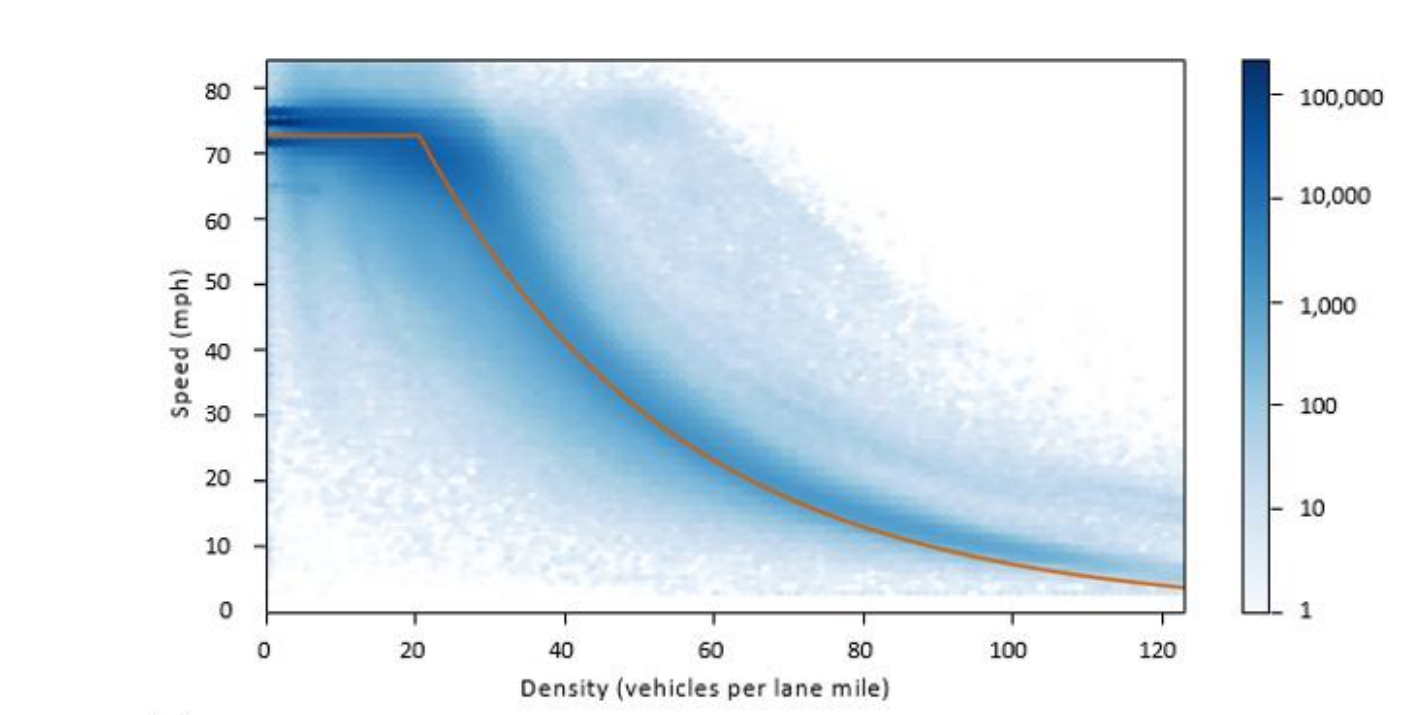
\includegraphics[width=\textwidth]{lit_bento_fig12a_speed_density.png}\\
\tiny Estimated speed--density curve (orange) over the 2017 data: flat to the kink, then falling. Source: Bento et al. (2023), Fig.~12a.
\end{column}
\begin{column}{0.42\textwidth}
\textbf{Above the kink}\\[0.3em]
\begin{tabular}{lc}
\toprule
OLS slope & $-0.0244$ \\
First stage & $0.638$ \\
KP F & $15.9$ \\
\textbf{IV slope} & $\mathbf{-0.0327}$ \\
\bottomrule
\end{tabular}\\[0.5em]
Each extra car per mile per lane cuts speed by \hl{3.3\%}.\\[0.3em]
Peak toll about \hl{33\textcent/mile}, near zero off-peak.
\end{column}
\end{columns}
\end{frame}

\begin{frame}[t]{Koch et al. (2023): method}
\small
\begin{columns}[T]
\begin{column}{0.5\textwidth}
\textbf{Berlin, 2017}
\begin{itemize}
\item INRIX GPS car trips, full year; trips clustered into drivers and routes
\item Log--log model:\\ $\ln(\text{time cost}) = \sigma \ln(\text{density}) + \dots$
\item Instrument: number of nearby incidents
\item Elasticity $\sigma$ estimated for each \hl{two-hour window}
\end{itemize}
\end{column}
\begin{column}{0.48\textwidth}
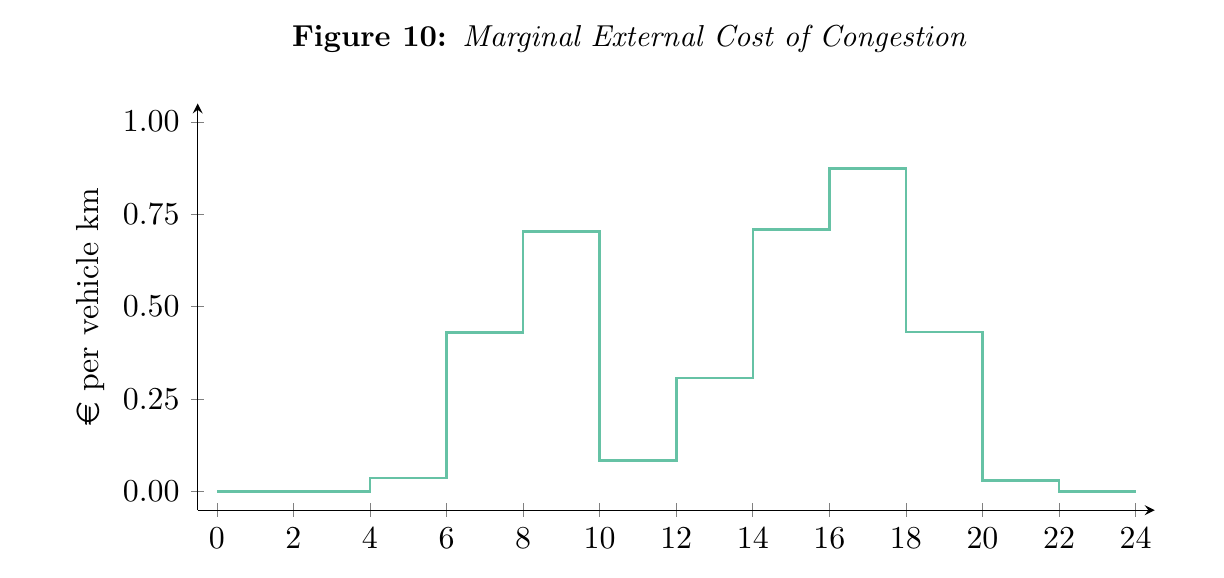
\includegraphics[width=\textwidth]{lit_koch_fig10_mec_by_hour.png}\\
\tiny Marginal external cost by two-hour window: high at the two peaks, near zero at night. Source: Koch et al. (2023), Fig.~10.
\end{column}
\end{columns}
\vspace{0.3em}
\begin{block}{What we take}
\small Two-hour windows, the elasticity $\sigma$, and $\text{MEC} = \frac{\sigma}{1-\sigma}\times$ average time cost. Not the GPS machine-learning steps (we have fixed sensors).
\end{block}
\end{frame}

\begin{frame}[t]{Koch et al. (2023): findings}
\small
\begin{columns}[T]
\begin{column}{0.56\textwidth}
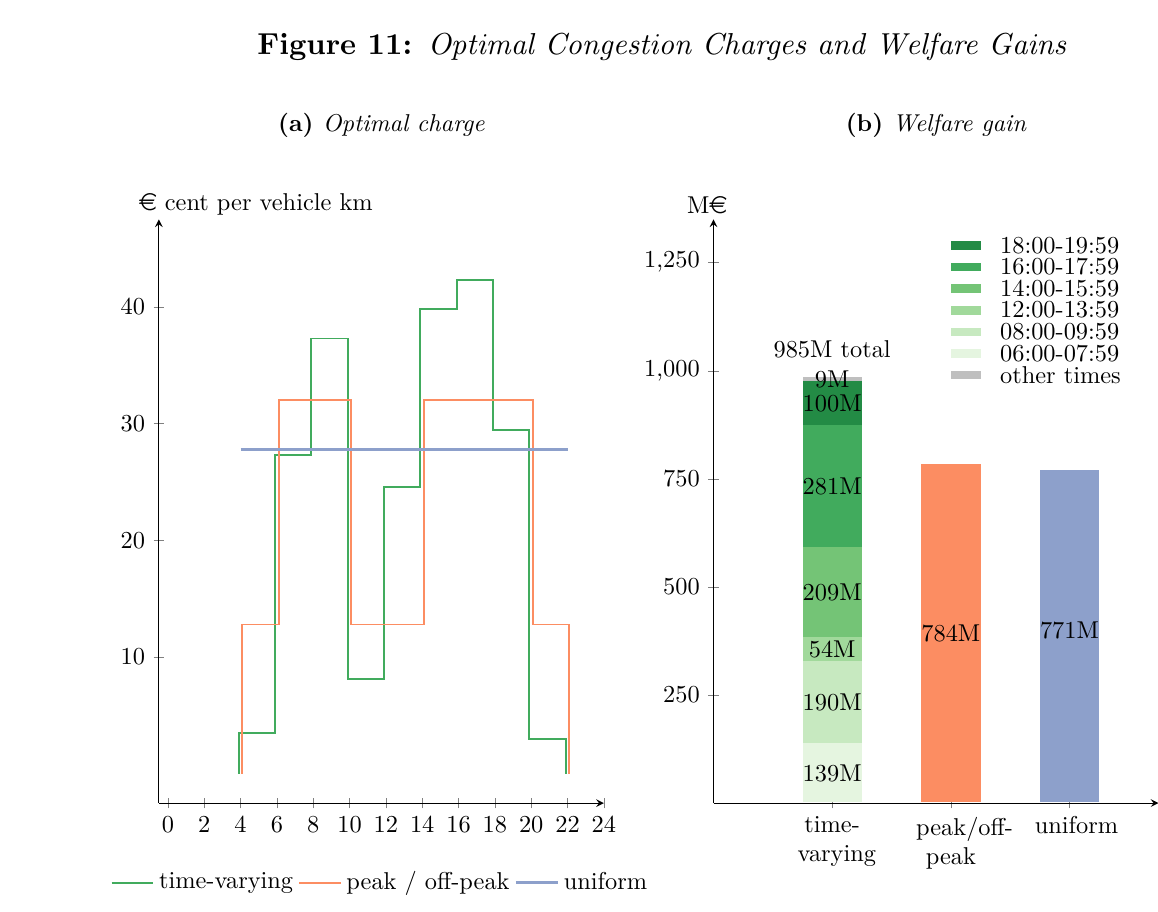
\includegraphics[width=\textwidth]{lit_koch_fig11_charges.png}\\
\tiny Optimal charges by time (green), peak/off-peak (orange) and uniform (blue), and the welfare gain of each. Source: Koch et al. (2023), Fig.~11.
\end{column}
\begin{column}{0.42\textwidth}
\begin{itemize}
\item Average $\sigma = 0.49$: 10\% more traffic $\Rightarrow$ 5\% slower trips
\item Peaks: 0.63 (8--10 am), \hl{0.67} (4--6 pm); quiet hours 0.08--0.17
\item MEC 3--87 euro cents/km
\item A uniform charge gets \hl{78\%} of the time-varying gain (771M vs 985M euros a year)
\end{itemize}
\end{column}
\end{columns}
\end{frame}

\begin{frame}[t]{The gap we address}
\begin{itemize}
\item Both papers find congestion costs \hl{more at rush hour}, but explain it differently:
\begin{itemize}
\item \textbf{Bento}: one curve for all hours; rush hour just has more cars.
\item \textbf{Koch}: elasticity estimated separately by clock time.
\end{itemize}
\item In Bento's semi-log form the elasticity is $\sigma = |\beta| \times D$, so it \hl{rises with density} automatically:
\end{itemize}
\begin{center}
\small
\begin{tabular}{lccc}
\toprule
Period (Bento, Table 4) & Slope & Mean density & Implied $\sigma$ \\
\midrule
AM peak & 0.0346 & 37.95 & 1.31 \\
PM peak & 0.0306 & 41.85 & 1.28 \\
Night & 0.0298 & 30.52 & 0.91 \\
\bottomrule
\end{tabular}
\end{center}
\begin{block}{Our contribution}
Test whether Koch-style hourly differences are just \hl{density in disguise}, on new 2026 data.
\end{block}
\end{frame}

%==========================================================
\section{Methodology and Data}
%==========================================================
\subsection{Data}
\begin{frame}[t]{Data sources}
\footnotesize
\begin{tabular}{L{2.6cm}L{7.6cm}}
\toprule
\textbf{Source} & \textbf{What it gives us} \\
\midrule
Caltrans PeMS, station-hour & Flow, occupancy, speed for every sensor station and hour, D7, Jan--Sep 2026: \hl{32.1M rows} \\
CHP incidents (via PeMS) & Every incident with time, type, freeway, direction, postmile, coordinates: \hl{102,544} in D7 \\
PeMS station metadata & Location, freeway, direction, lanes; ramp stations locate interchanges \\
NOAA GHCNh (hourly) & Temperature, wind, rain at LAX, Burbank, Long Beach, Van Nuys, Santa Monica, Camarillo \\
EIA & Weekly Los Angeles regular gasoline price \\
\bottomrule
\end{tabular}
\vspace{0.6em}
\begin{itemize}
\item Why 2026: the PeMS Clearinghouse now offers \hl{only 2026} data.
\item Key variable: \hl{density} $D = \dfrac{\text{flow per lane}}{\text{speed}}$ (cars per mile per lane).
\end{itemize}
\end{frame}

\subsection{Cleaning}
\begin{frame}[t]{Cleaning: rows we can trust}
\scriptsize
\begin{center}
\resizebox{\textwidth}{!}{%
\begin{tabular}{lrl}
\toprule
\textbf{Step} & \textbf{Rows left} & \textbf{Why} \\
\midrule
All rows, all lane types & 32,082,567 & \\
Main lanes only & 12,585,535 & HOV lanes and ramps behave differently \\
All detectors reporting (real readings) & 1,227,191 & PeMS fills broken sensors with estimates \\
All lanes reporting & 1,214,239 & otherwise per-lane density is wrong \\
Flow $> 0$ & 1,211,954 & 0 cars at 68 mph = faulty sensor \\
Drop 3 stuck stations & \hl{1,209,294} & speed never changes \\
\bottomrule
\end{tabular}}
\end{center}
\begin{itemize}
\item Rules 1--2 follow Bento et al.; the rest are our additions.
\item 51 hours with lane flow $> 2{,}500$ are \hl{kept and flagged}; every model is run with and without them.
\item Final sample: \hl{422 stations}; hours with an incident on the station's own stretch are excluded from regressions (as in Bento).
\end{itemize}
\end{frame}

\subsection{Identification}
\begin{frame}[t]{Why a simple regression is not enough}
\begin{itemize}
\item Speed and density move together, but not only because cars slow each other:
\begin{itemize}
\item a crash or rain lowers speed \emph{and} changes the number of cars;
\item drivers avoid roads they expect to be slow.
\end{itemize}
\item So OLS of speed on density mixes cause and effect.
\end{itemize}
\begin{block}{Instrumental variable (IV)}
Find something that adds cars to our road for a reason \hl{unrelated to our road's own conditions}: an incident on a nearby \hl{parallel freeway}. Drivers reroute onto our road.
\end{block}
\begin{itemize}
\item \textbf{Relevance:} the incident must raise density on our road (first stage, F statistic).
\item \textbf{Exclusion:} it must affect our speed \emph{only} through the extra cars.
\end{itemize}
\end{frame}

\begin{frame}[t]{Our instrument}
\begin{center}
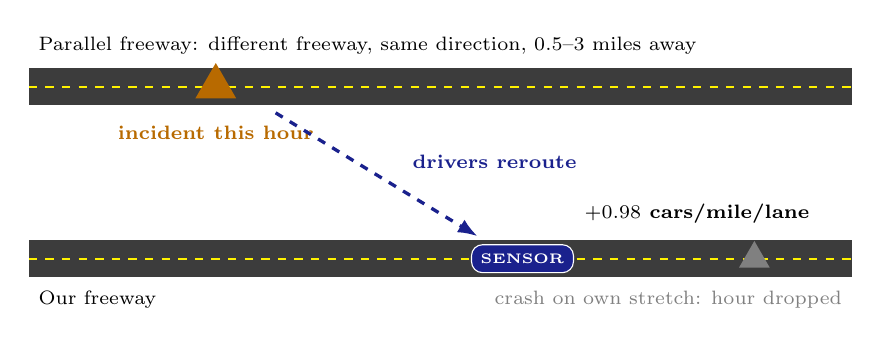
\begin{tikzpicture}[x=0.95cm, y=0.95cm, every node/.style={font=\scriptsize}]
  % parallel freeway
  \fill[Road] (0,2.6) rectangle (11,3.1);
  \draw[yellow, dashed, thick] (0,2.85) -- (11,2.85);
  \node[anchor=west] at (0,3.4) {Parallel freeway: different freeway, same direction, 0.5--3 miles away};
  \node[regular polygon, regular polygon sides=3, fill=Amber, minimum size=0.6cm, inner sep=0] at (2.5,2.85) {};
  \node[text=Amber, font=\scriptsize\bfseries, anchor=north] at (2.5,2.45) {incident this hour};
  % detour
  \draw[-{Latex[length=2.5mm]}, very thick, dashed, IITRBlue] (3.3,2.5) .. controls (4.6,1.7) .. (6.0,0.85);
  \node[text=IITRBlue, font=\scriptsize\bfseries, anchor=west] at (5.0,1.85) {drivers reroute};
  % our freeway
  \fill[Road] (0,0.3) rectangle (11,0.8);
  \draw[yellow, dashed, thick] (0,0.55) -- (11,0.55);
  \node[anchor=west] at (0,0.0) {Our freeway};
  \node[draw=white, fill=IITRBlue, text=white, font=\tiny\bfseries, rounded corners] at (6.6,0.55) {SENSOR};
  \node[anchor=west, font=\scriptsize\bfseries] at (7.3,1.15) {$+0.98$ cars/mile/lane};
  \node[regular polygon, regular polygon sides=3, fill=gray, minimum size=0.45cm, inner sep=0] at (9.7,0.55) {};
  \node[text=gray, anchor=east] at (11,0.0) {crash on own stretch: hour dropped};
\end{tikzpicture}
\end{center}
\small
\begin{itemize}
\item Bento et al. used \hl{Google Maps alternative routes} for real commutes; we used \hl{parallel freeways} to finish in time (our simplification).
\item Each incident is matched to the nearest sensor within 1 mile on its freeway and direction (94\% matched).
\item 159 of 422 stations have a parallel freeway nearby; 1.3\% of station-hours are treated.
\end{itemize}
\end{frame}

\subsection{Regressions}
\begin{frame}[t]{Estimation}
\small
\textbf{1. Kink search} (for $b = 1,\dots,50$; keep the lowest AIC):
\[
\ln v_{it} = \beta\,(D_{it}-b)\,\mathbf{1}[D_{it}>b] + X_{it}'\delta + \alpha_i + \tau_{h(t)} + \omega_{d(t)} + \mu_{m(t)} + \varepsilon_{it}
\]
\textbf{2. First stage} (split by whether a station's usual density is above the kink):
\[
D_{it} = \gamma\, Z_{it} + X_{it}'\delta + \alpha_i + \tau_h + \omega_d + \mu_m + u_{it}
\]
\textbf{3. Second stage (2SLS):}
\[
\ln v_{it} = \beta\, \widehat{D}_{it} + X_{it}'\delta + \alpha_i + \tau_h + \omega_d + \mu_m + \varepsilon_{it}
\]
\begin{itemize}
\item $Z_{it}$: incident on a parallel freeway in hour $t$; $X_{it}$: temperature, temp$^2$, wind, rain, gas price, D7 vehicle-miles.
\item Fixed effects: station $\alpha_i$, hour $\tau$, weekday $\omega$, month $\mu$ (each station compared with itself).
\item Standard errors clustered two ways, by station and by date.
\end{itemize}
\end{frame}

\begin{frame}[t]{Time-of-day test and welfare model}
\footnotesize
\textbf{Does the curve shift by hour?}
\begin{itemize}
\item Slope $\beta_k$ and kink $b_k$ estimated separately for each two-hour window $k$; Wald test of equal slopes.
\item Koch-style $\sigma_k$ (log--log, per window) vs the $\sigma$ that \hl{one pooled curve} predicts at each window's densities: $\sigma = |\beta|\,D\,\mathbf{1}[D>b]$.
\end{itemize}
\textbf{Tolls and welfare} (Bento's model):
\[
v(D)=\begin{cases} v_f & D\le b\\ v_f\,e^{\beta(D-b)} & D>b\end{cases},\qquad q = D\,v(D),\qquad \text{MEC} = \frac{\text{VOT}}{v}\cdot\frac{\sigma}{1-\sigma}
\]
\begin{itemize}
\item Past peak flow, extra cars only queue (Verhoef 2001). Free flow = 2--4 am average (67.4 mph).
\item VOT \$24.30/vehicle-hour; demand elasticity $-2.0$ (range $-0.67$ to $-2.0$).
\item 9,931 station $\times$ hour cases; best toll for four policies: \hl{ideal} (station $\times$ hour), \hl{hourly}, \hl{two-hour}, \hl{flat}.
\end{itemize}
\end{frame}

%==========================================================
\section{EDA and Results}
%==========================================================
\subsection{Exploratory analysis}
\begin{frame}[t]{EDA 1: most sensors are broken}
\begin{center}
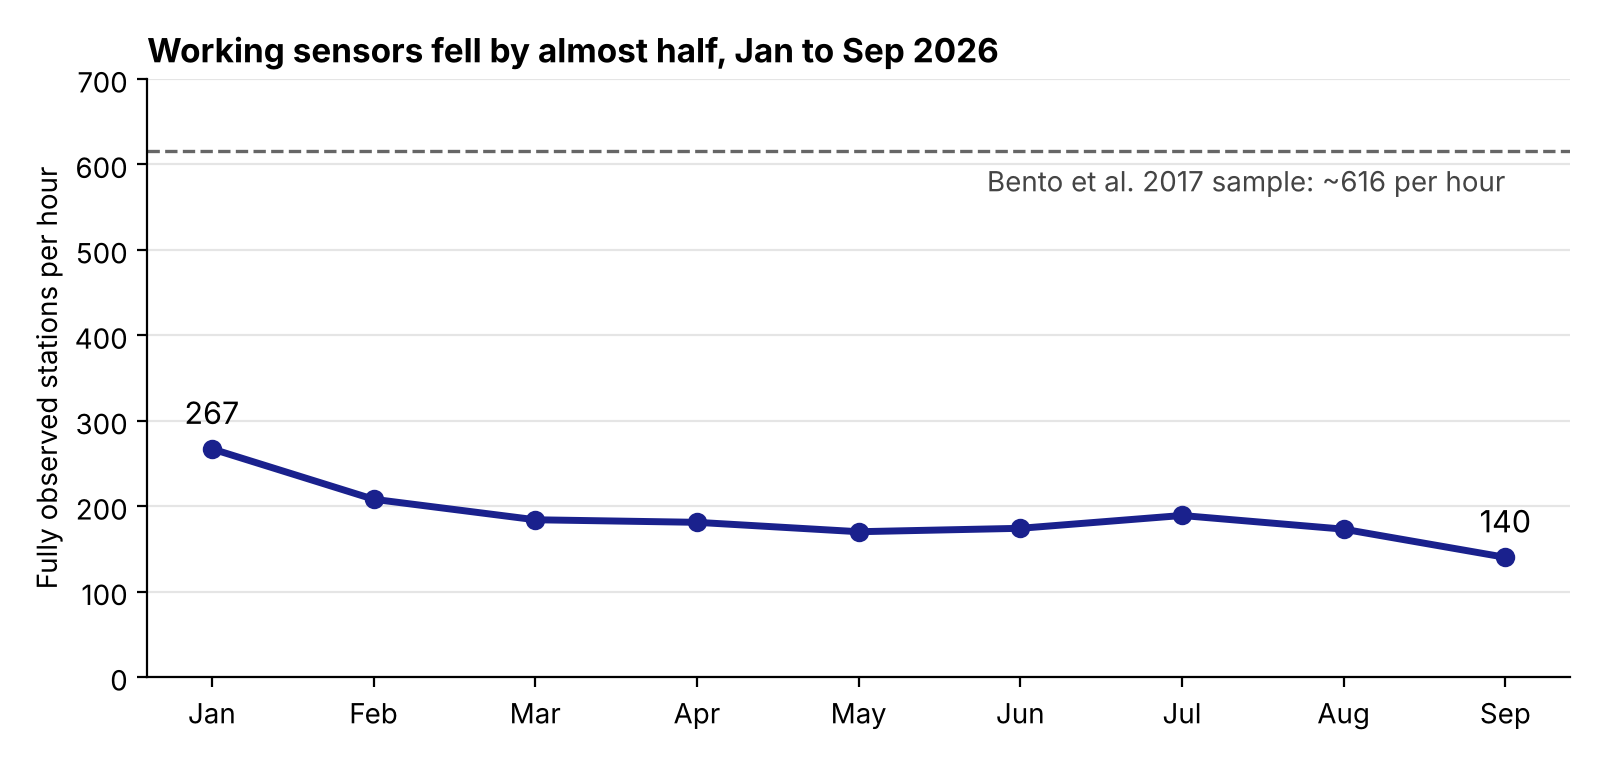
\includegraphics[width=0.85\textwidth]{coverage_by_month.png}
\end{center}
\small
\begin{itemize}
\item \hl{86\%} of mainline station-hours are PeMS estimates, not real readings; 1,572 of 1,936 stations had no real readings in Jul--Sep.
\item Usable: 1.23M station-hours from 430 stations (Bento: 1.36M from 1,318).
\end{itemize}
\end{frame}

\begin{frame}[t]{EDA 2: estimates and coverage}
\begin{columns}[T]
\begin{column}{0.5\textwidth}
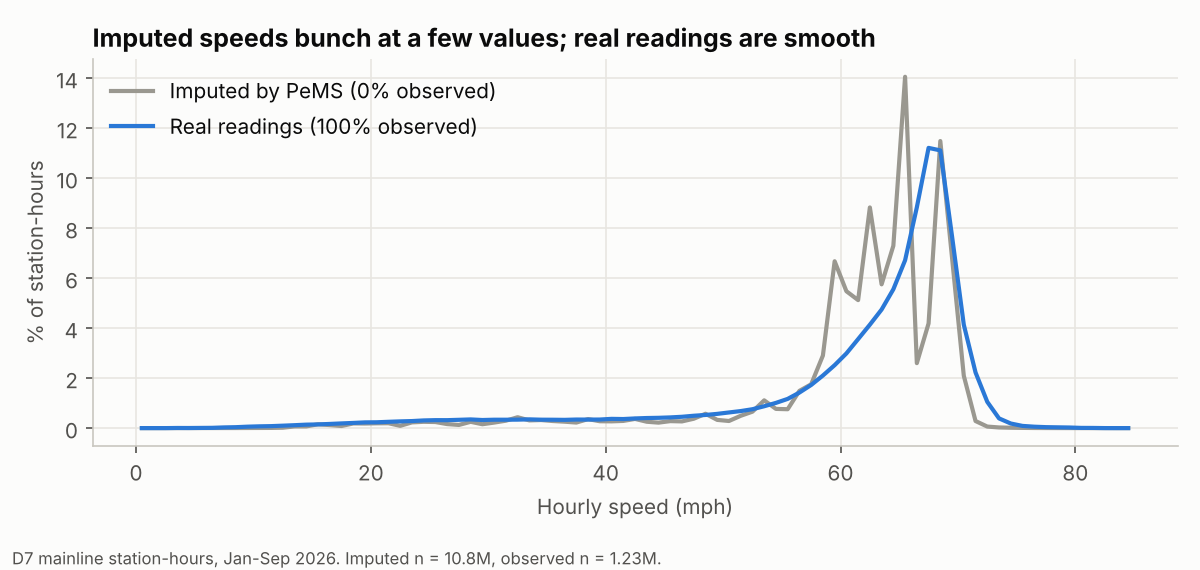
\includegraphics[width=\textwidth]{fig3_imputed_vs_observed_speed.png}
\scriptsize Imputed speeds bunch at a few values $\Rightarrow$ excluded.
\end{column}
\begin{column}{0.5\textwidth}
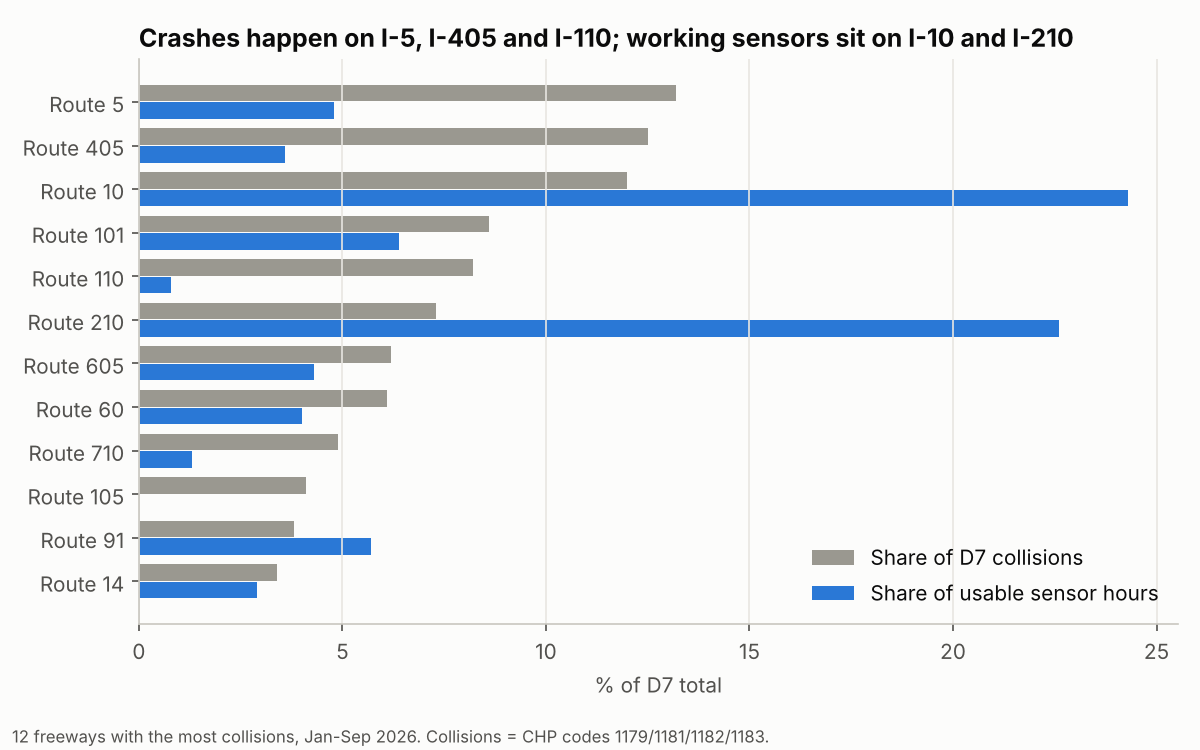
\includegraphics[width=\textwidth]{fig4_freeway_coverage_vs_collisions.png}
\scriptsize I-10 and I-210 hold 47\% of usable hours but 19\% of collisions; I-5, I-405, I-110: 34\% of collisions, 9\% of hours.
\end{column}
\end{columns}
\end{frame}

\begin{frame}[t]{EDA 3: the speed--density curve has a kink}
\begin{center}
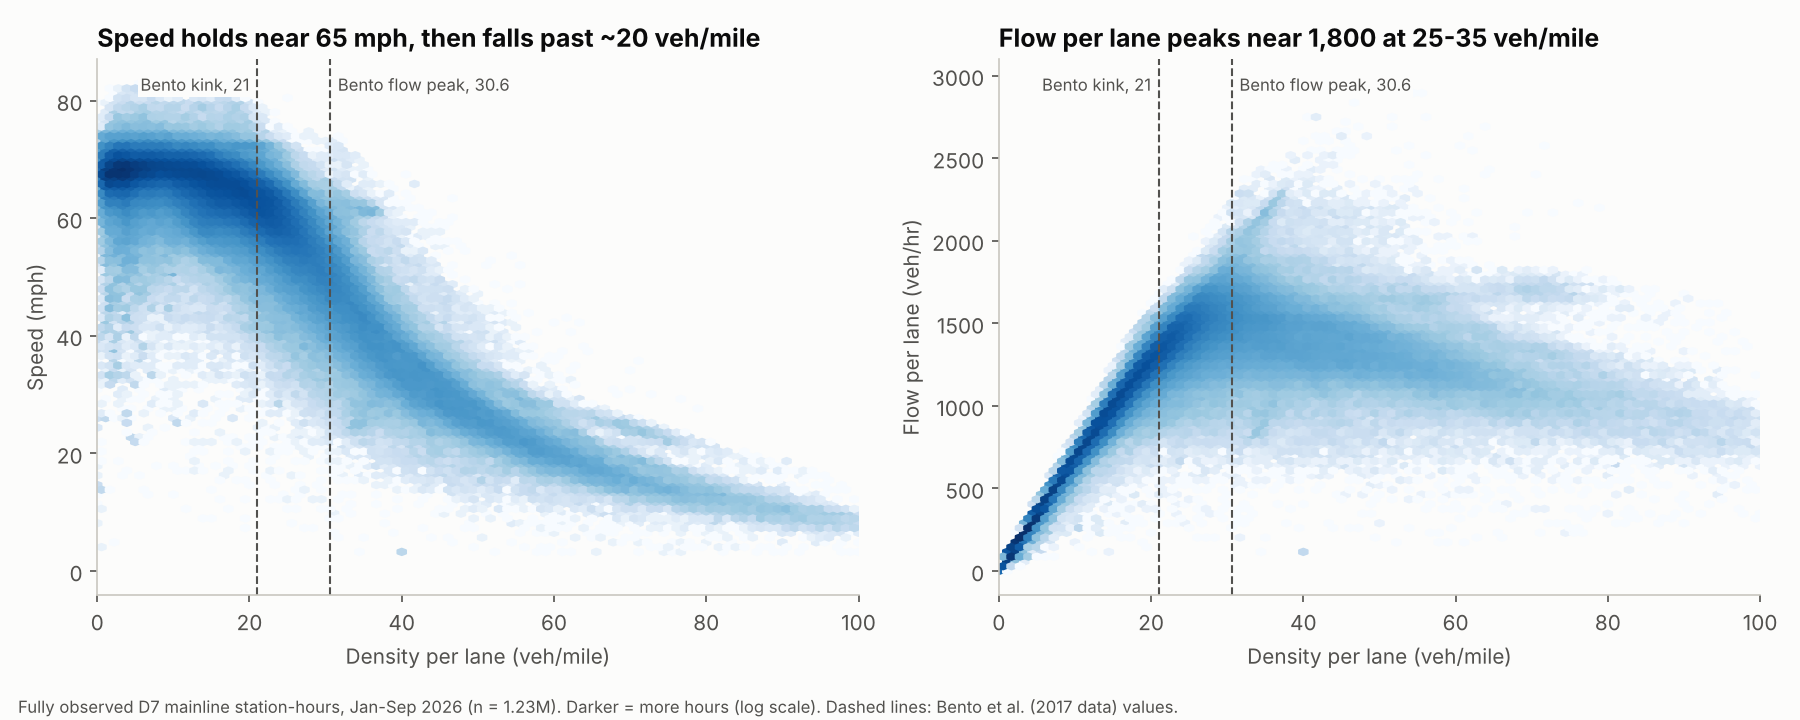
\includegraphics[width=\textwidth]{fig1_fundamental_diagram.png}
\end{center}
\small
\begin{itemize}
\item Speed holds near 65--68 mph, then falls past about 20 cars/mile/lane; flow peaks near 1,800 per lane.
\item Parallel bands = different stations follow different curves $\Rightarrow$ station fixed effects are essential.
\end{itemize}
\end{frame}

\begin{frame}[t]{EDA 4: rush hour in the data}
\begin{center}
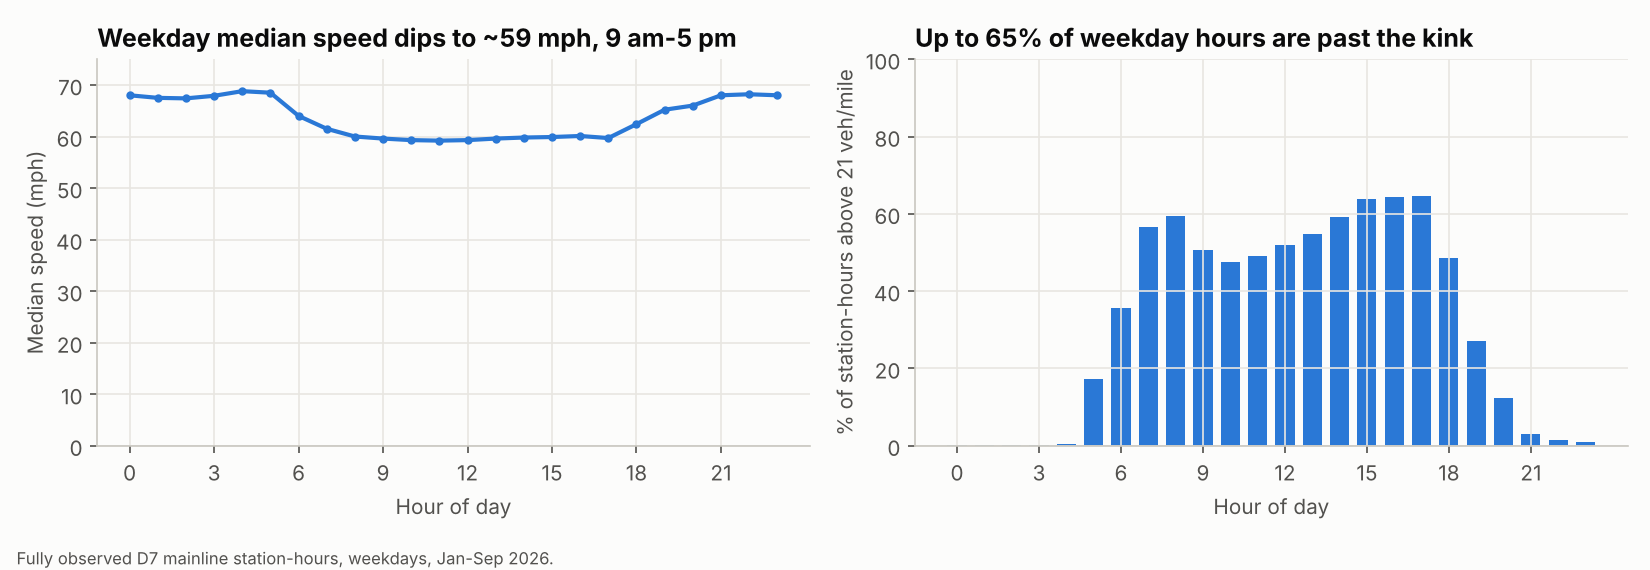
\includegraphics[width=\textwidth]{fig2_hour_of_day.png}
\end{center}
\small
Weekday median speed falls from about 68 mph at night to about 59 mph in the day; at 5 pm, 65\% of station-hours are past the kink.
\end{frame}

\subsection{Results}
\begin{frame}[t]{Result 1: the kink is at 19}
\begin{center}
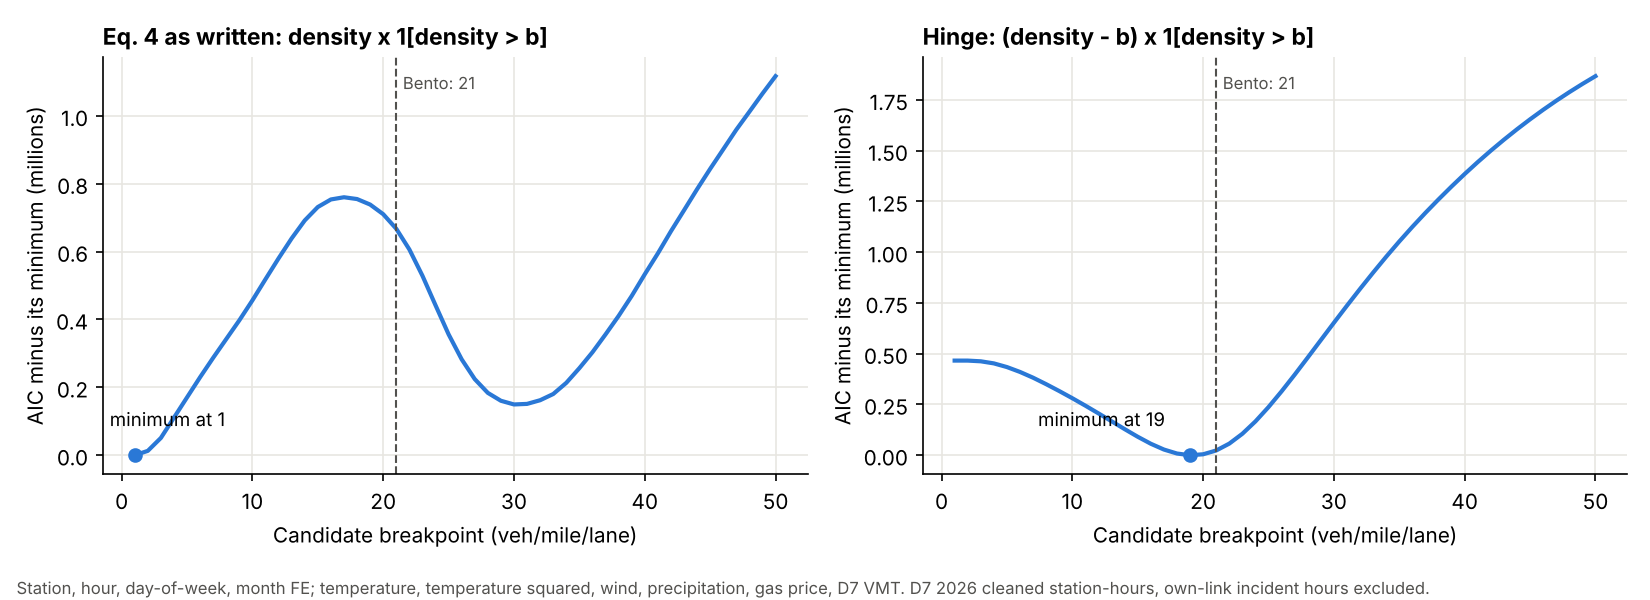
\includegraphics[width=\textwidth]{breakpoint_search.png}
\end{center}
\small
\begin{itemize}
\item Hinge form picks \hl{19} cars/mile/lane (Bento: 21), slope $-0.028$.
\item Bento's equation \emph{as printed} finds no kink (minimum at 1) $\Rightarrow$ the paper's equation likely has a typo.
\end{itemize}
\end{frame}

\begin{frame}[t]{Result 2: OLS vs IV}
\small
\begin{center}
\begin{tabular}{lcccc}
\toprule
 & \multicolumn{2}{c}{Below the kink} & \multicolumn{2}{c}{Above the kink} \\
 & Ours & Bento & Ours & Bento \\
\midrule
OLS slope & $-0.0113$ & $-0.0044$ & $-0.0270$ & $-0.0244$ \\
 & (0.0008) & & (0.0004) & \\
First stage & 0.128 & 0.033 & 0.984 & 0.638 \\
 & (0.070) & & (0.293) & \\
First-stage F & 3.4 & 5.4 & 11.3 & 15.9 \\
\textbf{IV slope} & $-0.0235$ & $-0.0196$ & $\mathbf{-0.0378}$ & $\mathbf{-0.0327}$ \\
 & (0.0116) & & (0.0047) & \\
N & 747,013 & & 442,731 & \\
\bottomrule
\end{tabular}
\end{center}
\begin{itemize}
\item Above the kink, each extra car per mile per lane cuts speed by \hl{3.8\%} (Bento 3.3\%).
\item OLS understates the effect by about 30\%. Below the kink the instrument is weak (as in Bento).
\end{itemize}
\end{frame}

\begin{frame}[t]{Result 3: robustness (above the kink)}
\small
\begin{center}
\begin{tabular}{lcc}
\toprule
Specification & IV slope & First-stage F \\
\midrule
Main (all incidents) & $-0.0378$ & 11.3 \\
Without high-flow rows ($>2{,}500$) & $-0.0378$ & 11.3 \\
Collisions only & $-0.0353$ & 14.9 \\
Collisions + hit-and-run & $-0.0358$ & 15.6 \\
Holidays excluded & $-0.0380$ & 10.0 \\
Bento's kink (21) & $-0.0379$ & 11.0 \\
Balanced panel (151 stations) & $-0.0328$ & 6.8 \\
\bottomrule
\end{tabular}
\end{center}
\begin{itemize}
\item Every specification gives \hl{3.3\%--3.8\%} per extra car.
\item Only the balanced panel has a weak first stage (smaller sample).
\end{itemize}
\end{frame}

\begin{frame}[t]{Result 4: the curve does not shift by hour}
\begin{center}
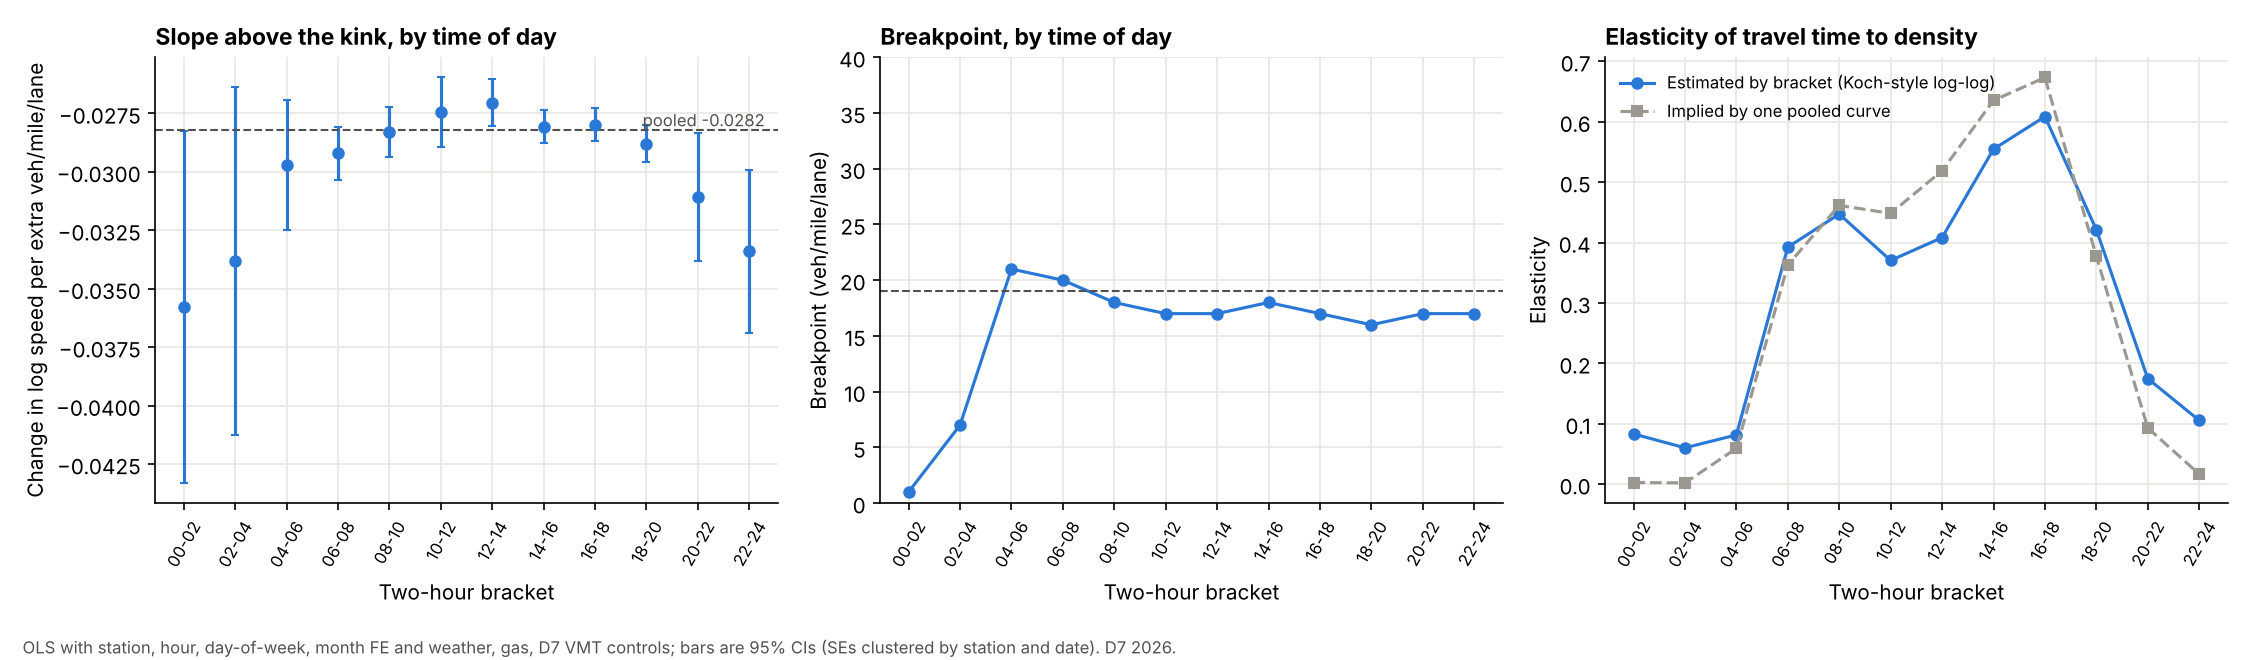
\includegraphics[width=\textwidth]{time_of_day.png}
\end{center}
\scriptsize
\begin{itemize}
\item 6 am--8 pm: slope $-0.027$ to $-0.029$ in every window; kink 16--21. (Wald test rejects exact equality with 1.2M observations, but the gaps are small and largest at night, where almost no hours are congested.)
\item Koch-style elasticity per window tracks the \hl{single-curve prediction} (correlation 0.98); 4--6 pm: 0.61 vs Koch's 0.67.
\end{itemize}
\end{frame}

\begin{frame}[t]{Result 5: tolls and welfare}
\begin{columns}[T]
\begin{column}{0.56\textwidth}
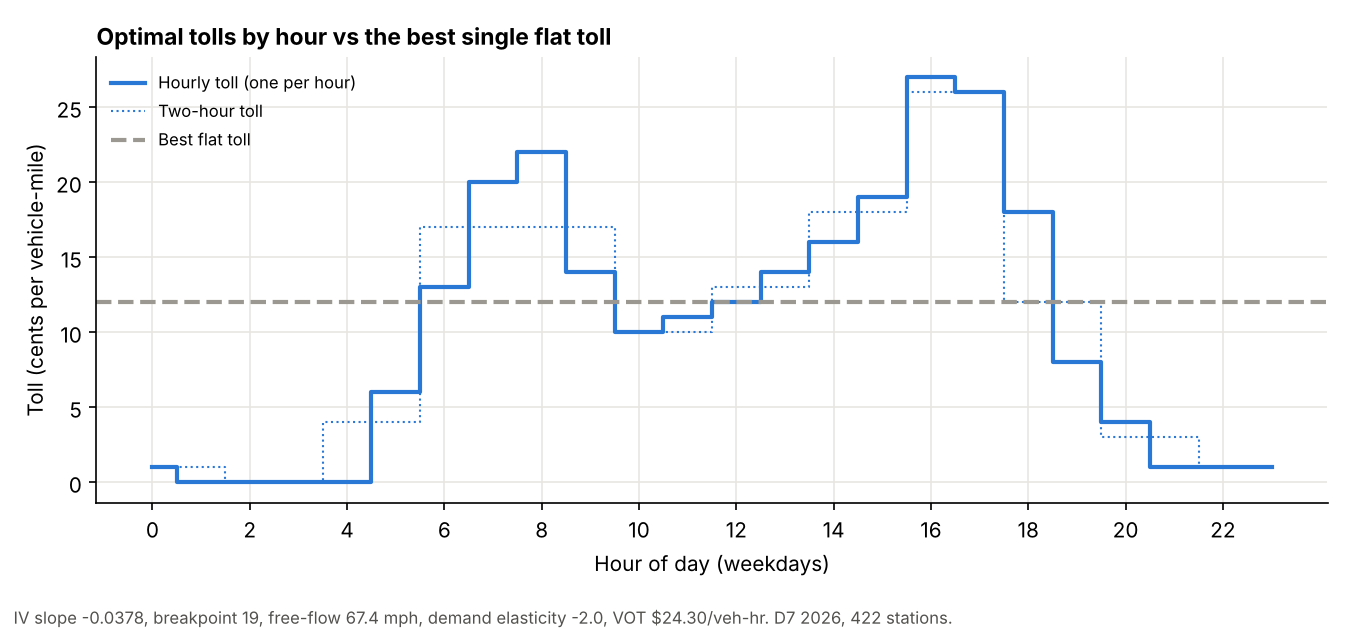
\includegraphics[width=\textwidth]{welfare.png}
\end{column}
\begin{column}{0.42\textwidth}
\scriptsize
\begin{tabular}{lcc}
\toprule
Policy & Gain (\textcent/veh-mi) & Share \\
\midrule
Ideal (station $\times$ hour) & 11.8 & 100\% \\
Hourly & 3.4 & 29\% \\
Two-hour & 3.3 & 28\% \\
Flat (12\textcent) & 2.7 & 23\% \\
\bottomrule
\end{tabular}
\end{column}
\end{columns}
\small
\begin{itemize}
\item Peak hourly toll \hl{27\textcent/mile} at 4--5 pm (Bento 33\textcent), 22\textcent{} at 8--9 am, about 0 at night.
\item A flat toll gets \hl{80\%} of the hourly gain (80--83\% under every VOT and elasticity tried).
\item Clock-based tolls capture \hl{under 30\%} of the ideal; the rest needs pricing by \emph{where} the road is crowded.
\end{itemize}
\end{frame}

%==========================================================
\section{Comparison with Literature}
%==========================================================
\begin{frame}[t]{What is different in our study}
\footnotesize
\begin{tabular}{L{2.3cm}L{3.9cm}L{3.9cm}}
\toprule
 & \textbf{Bento et al. (2023)} & \textbf{This project} \\
\midrule
Data year & 2017 (Aug, 92 days) & 2026 (Jan--Sep) \\
Sensors & 1,318 stations & 422 stations (most sensors now broken) \\
Instrument & Crash on Google Maps alternative route & Incident on parallel freeway, 0.5--3 miles \\
Kink form & As printed: jump at kink & Hinge: speed falls smoothly from kink \\
Weather & NOAA ISD-Lite & NOAA GHCNh (ISD-Lite retired 2025) \\
Time of day & 4 broad periods & 12 two-hour windows + Koch elasticities \\
Flat vs hourly & Not computed & True second-best flat toll \\
\bottomrule
\end{tabular}
\end{frame}

\begin{frame}[t]{How our numbers compare}
\small
\begin{center}
\resizebox{\textwidth}{!}{%
\begin{tabular}{lccc}
\toprule
 & \textbf{Ours (LA 2026)} & \textbf{Bento (LA 2017)} & \textbf{Koch (Berlin 2017)} \\
\midrule
Kink (cars/mile/lane) & 19 & 21 & -- \\
Speed lost per extra car & 3.8\% & 3.3\% & -- \\
OLS vs IV & IV 40\% larger & IV 34\% larger & IV 7$\times$ larger \\
Peak elasticity $\sigma$ & 0.61 (4--6 pm) & 0.69 at kink & 0.67 (4--6 pm) \\
Peak toll & 27\textcent/mile & 33\textcent/mile & up to 42 euro c/km \\
Flat vs time-varying & 80\% & -- & 78\% \\
\bottomrule
\end{tabular}}
\end{center}
\begin{itemize}
\item Despite new data and a simpler instrument, we land \hl{close to Bento}.
\item We reproduce Koch's hourly pattern, but show it is explained by \hl{density}, not the clock.
\end{itemize}
\end{frame}

\begin{frame}[t]{Results at a glance}
\begin{center}
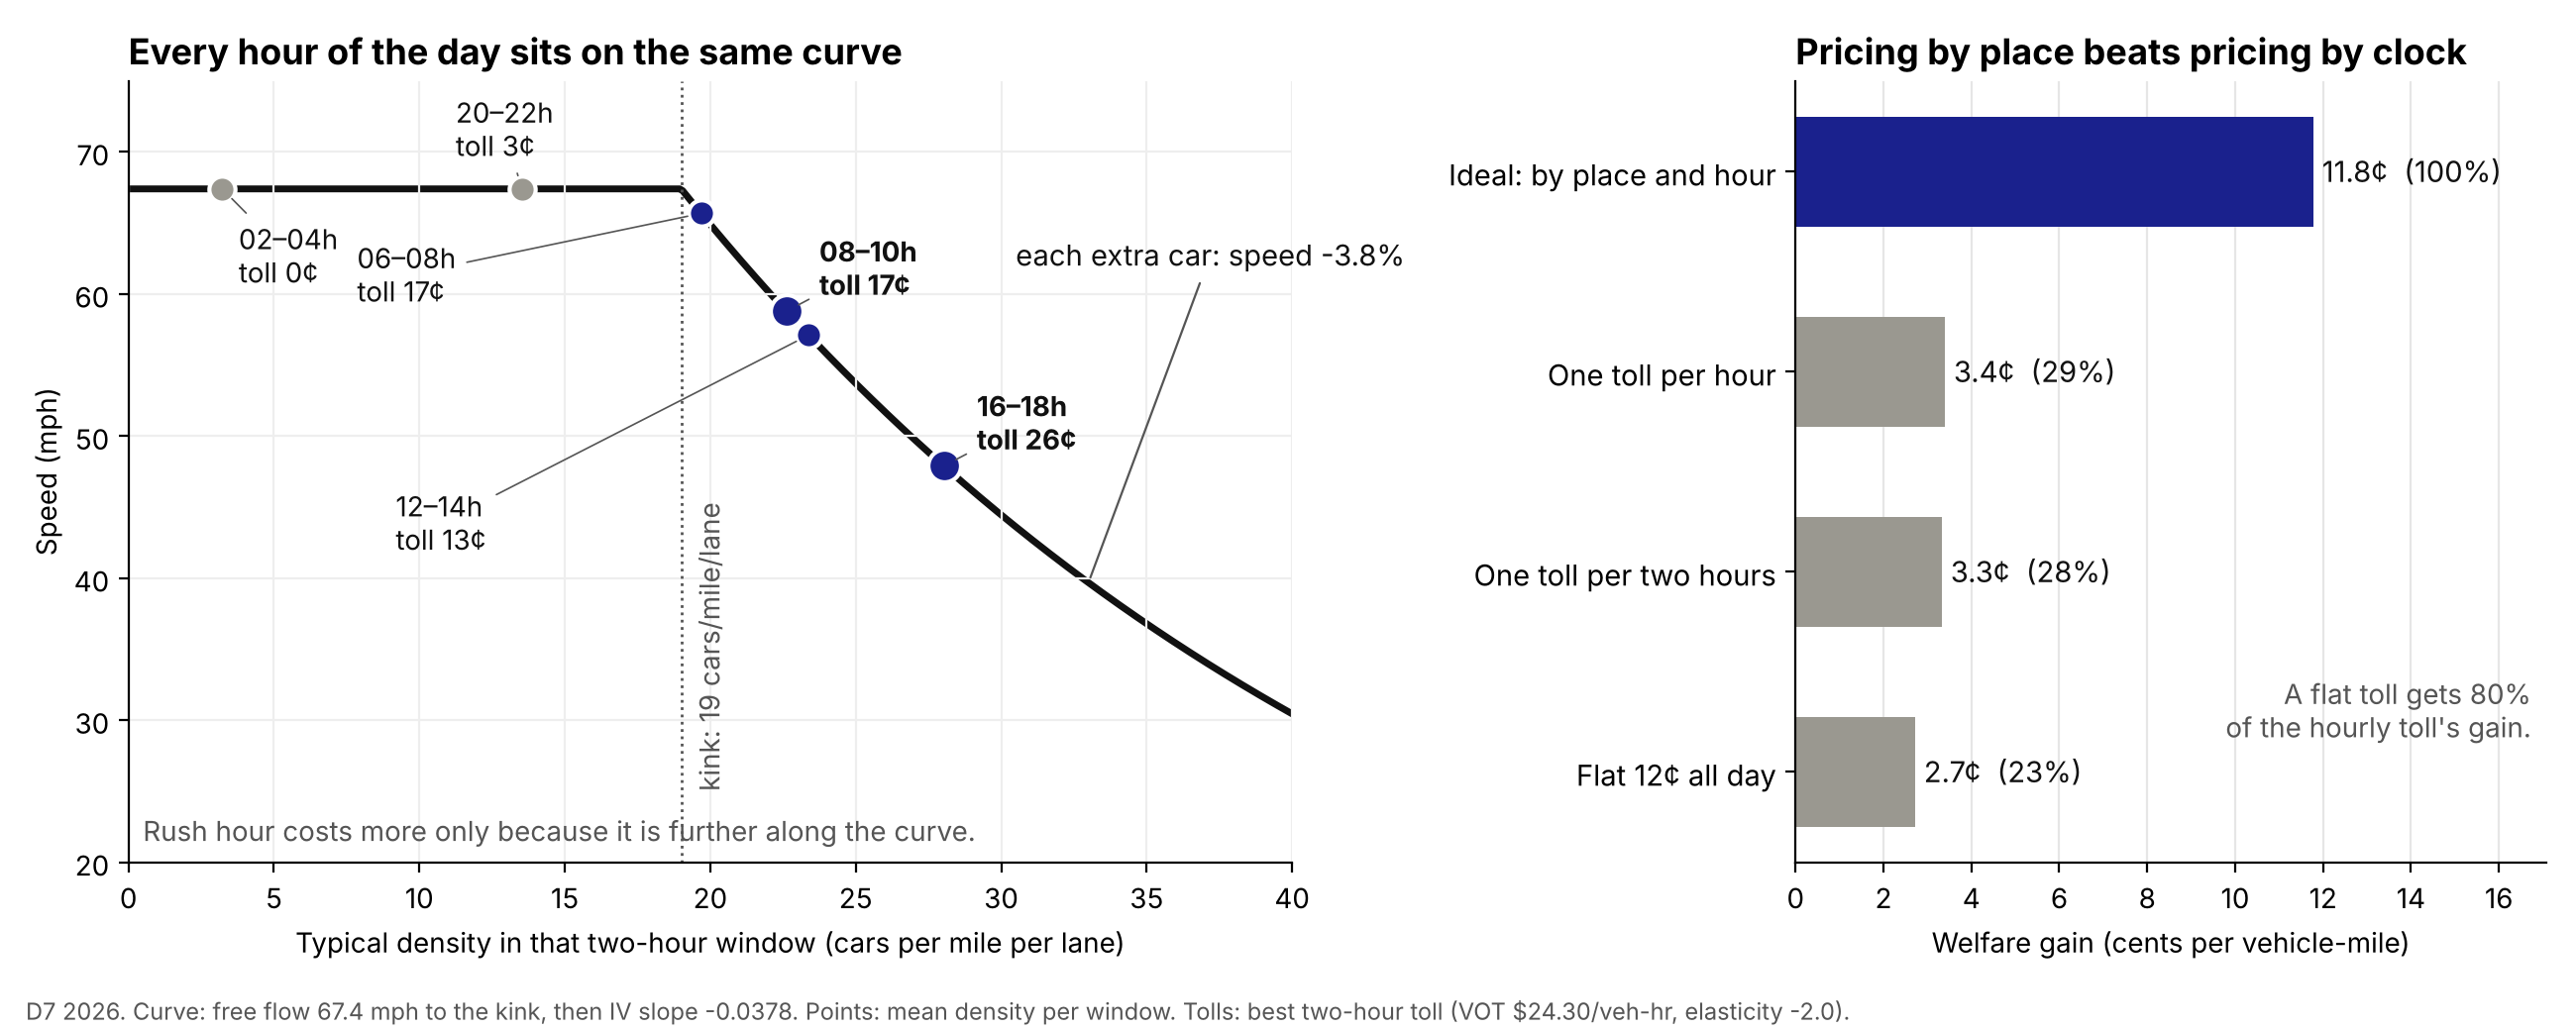
\includegraphics[width=\textwidth]{results_at_a_glance.png}
\end{center}
\small
\begin{itemize}
\item \textbf{Left:} each two-hour window, placed at its typical density on our \emph{one} estimated curve. Night sits on the flat part (no toll); the peaks sit furthest down the slope (highest tolls).
\item \textbf{Right:} clock-based tolls capture under 30\% of the gain from pricing each place by how crowded it is.
\end{itemize}
\end{frame}

%==========================================================
\section{Conclusion}
%==========================================================
\begin{frame}[t]{Conclusion}
\begin{block}{Findings}
\begin{itemize}
\item Past 19 cars per mile per lane, each extra car cuts speed by about \hl{3.8\%}.
\item The curve is the \hl{same at every busy hour}: rush hour costs more because it is crowded, not because of the clock.
\item Best hourly toll peaks at \hl{27\textcent/mile}; a flat 12\textcent{} toll gets 80\% of that gain; both miss over 70\% of the gain from pricing by real-time crowding.
\end{itemize}
\end{block}
\begin{block}{Policy}
Price congestion by \hl{measured density} (dynamic, location-specific) rather than a fixed hour-of-day schedule.
\end{block}
\end{frame}

\begin{frame}[t]{Limitations and future work}
\small
\begin{itemize}
\item \textbf{Instrument:} simplified (parallel freeways, not real commute routes); covers 159 stations; moderate strength (F = 11.3).
\item \textbf{Sensors:} only 422 working stations, concentrated on I-10 and I-210, and falling through the year.
\item \textbf{No validation on Bento's 2017 data}: method differences and real 2017--2026 change cannot be fully separated.
\item \textbf{Assumed parameters:} value of time and demand elasticity (we report ranges).
\item \textbf{Static model:} no network rerouting, no change in departure times.
\end{itemize}
\vspace{0.3em}
\textbf{Future work:} Google Maps routes from LODES commutes; validation on Bento's replication data; San Francisco Bay Area (District 4) with rain as a curve shifter.
\end{frame}

%%%%%%%%%%%%% Thanks Slide %%%%%%%%%%%%%%%%%
{\usebackgroundtemplate{\includegraphics[width=\paperwidth,height=\paperheight]{white_bg.png}}
\begin{frame}[plain,c]
\begin{center}
{\color{IITRBlue}\LARGE \underline{Thanks.}}
\end{center}
\end{frame}
}
%%%%%%%%%%%%%%%%%%%%%%%%%%%%%%%%%%%%%%%%%%%

%==========================================================
\section{References}
%==========================================================
\begin{frame}[t]{References}
\scriptsize
\begin{itemize}
\item Bento, A., Hall, J. D., \& Heilmann, K. (2023). \emph{Evaluating Alternative Strategies for Traffic Reduction in Los Angeles}. National Center for Sustainable Transportation, Report NCST-USC-RR-23-28. \url{https://doi.org/10.7922/G2JW8C6H}
\item Koch, N., Ritter, N., Rohlf, A., \& Thies, F. (2023). \emph{Machine Learning from Big GPS Data about the Heterogeneous Costs of Congestion}. SSRN Working Paper 4526796. \url{https://doi.org/10.2139/ssrn.4526796}
\item Parry, I. W. H. (2008). \emph{Pricing Urban Congestion}. Resources for the Future Discussion Paper 08-35; published in \emph{Annual Review of Resource Economics}, 1 (2009).
\item Verhoef, E. T. (2001). An integrated dynamic model of road traffic congestion based on simple car-following theory. \emph{Journal of Urban Economics}, 49(3), 505--529.
\item Anderson, M. L. (2014). Subways, strikes, and slowdowns: The impacts of public transit on traffic congestion. \emph{American Economic Review}, 104(9), 2763--2796.
\item Caltrans Performance Measurement System (PeMS), District 7 station-hour data, station metadata and CHP incidents, 2026. \url{https://pems.dot.ca.gov}
\item NOAA National Centers for Environmental Information, Global Historical Climatology Network hourly (GHCNh), 2026.
\item U.S. Energy Information Administration, Los Angeles regular gasoline retail prices, weekly, 2026.
\end{itemize}
\end{frame}

\end{document}
